\begin{pastexam}[label={px:nccu-108-dsa-01}]{政大資科所 108 學年度 第 1 題}
（問答）

(10\%) Use Kruskal's algorithm to find the minimum spanning tree of the following graph.
\begin{center}
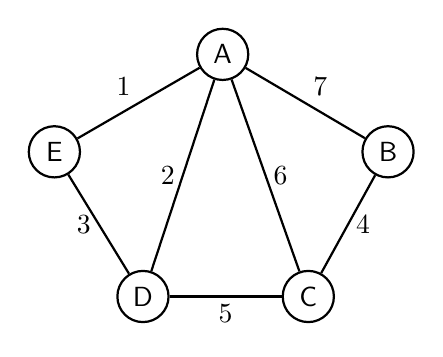
\begin{tikzpicture}[x=0.75cm,y=0.75cm,thick,
  v/.style={circle,draw,minimum size=6.5mm,inner sep=0pt,font=\sffamily},lab/.style={inner sep=2.5pt}]
\node[v] (A) at (4.85,-0.8) {A}; \node[v] (E) at (2.0,-2.45) {E}; \node[v] (B) at (7.65,-2.45) {B};
\node[v] (D) at (3.5,-4.9) {D}; \node[v] (C) at (6.3,-4.9) {C};
\draw (A) -- node[lab,above left] {1} (E);
\draw (A) -- node[lab,above right] {7} (B);
\draw (A) -- node[lab,left] {2} (D);
\draw (A) -- node[lab,right] {6} (C);
\draw (E) -- node[lab,left] {3} (D);
\draw (B) -- node[lab,right] {4} (C);
\draw (D) -- node[lab,below] {5} (C);
\end{tikzpicture}
\end{center}
\end{pastexam}

\begin{pastsoln}
答案：最小生成樹由 A--E（$1$）、A--D（$2$）、B--C（$4$）、D--C（$5$）四條邊組成，總權重 $12$。

\textbf{Kruskal}（資結書第~24.2~節）：所有邊依權重由小到大看，兩端已經在同一個集合（加進來會成環）
就跳過，否則加入並合併兩個集合。 $5$ 個頂點，加滿 $4$ 條邊就完成。 邊的權重 $1$--$7$ 全部不同，所以
最小生成樹只有一棵（資結書定理~24.4）。
\begin{center}
\begin{tabular}{cclll}
\toprule
權重 & 邊 & 結果 & 第幾條 & 加入後的集合 \\
\midrule
1 & A--E & 加入 & 1 & $\{A, E\}$, $\{B\}$, $\{C\}$, $\{D\}$ \\
2 & A--D & 加入 & 2 & $\{A, D, E\}$, $\{B\}$, $\{C\}$ \\
3 & E--D & 跳過（E、D 同集合） & & \\
4 & B--C & 加入 & 3 & $\{A, D, E\}$, $\{B, C\}$ \\
5 & D--C & 加入 & 4 & $\{A, B, C, D, E\}$ \\
6 & A--C & 不用再看（已有 $4$ 條） & & \\
7 & A--B & （同上） & & \\
\bottomrule
\end{tabular}
\end{center}

最小生成樹（粗線）：
\begin{center}
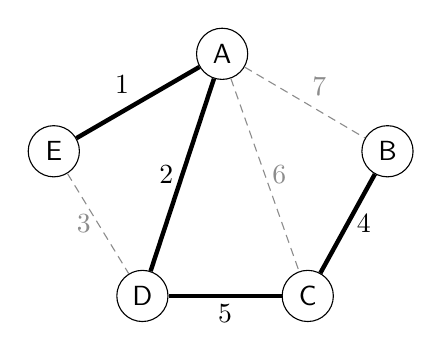
\begin{tikzpicture}[x=0.75cm,y=0.75cm,
  v/.style={circle,draw,minimum size=6.5mm,inner sep=0pt,font=\sffamily},lab/.style={inner sep=2.5pt},
  t/.style={line width=1.6pt},n/.style={densely dashed,black!45}]
\node[v] (A) at (4.85,-0.8) {A}; \node[v] (E) at (2.0,-2.45) {E}; \node[v] (B) at (7.65,-2.45) {B};
\node[v] (D) at (3.5,-4.9) {D}; \node[v] (C) at (6.3,-4.9) {C};
\draw[t] (A) -- node[lab,above left] {1} (E);
\draw[n] (A) -- node[lab,above right] {7} (B);
\draw[t] (A) -- node[lab,left] {2} (D);
\draw[n] (A) -- node[lab,right] {6} (C);
\draw[n] (E) -- node[lab,left] {3} (D);
\draw[t] (B) -- node[lab,right] {4} (C);
\draw[t] (D) -- node[lab,below] {5} (C);
\end{tikzpicture}
\end{center}
總權重 $1 + 2 + 4 + 5 = 12$。 檢查：沒選的邊 E--D（$3$）、A--C（$6$）、A--B（$7$）各自和樹上的路徑
成環，而且都是那個環上最重的邊（E--A--D 的 $1, 2$；A--D--C 的 $2, 5$；A--D--C--B 的 $2, 5, 4$），由
環性質（資結書定理~24.3）它們都不在最小生成樹裡。 次小的生成樹是把 D--C 換成 A--C，權重 $13$。
\end{pastsoln}
